\documentclass[12pt]{article}

% ----- Preamble
\usepackage[utf8]{inputenc} % police encodee en latin1=iso8859-1=Windows Latin 1 %
\usepackage[french]{babel} % police fr %
\usepackage{hyperref} % pour les references %
\usepackage{amsmath} % pour les formules de maths %
\usepackage{amssymb} % pour les symboles maths %
\usepackage{amsthm} % pour la mise en forme des theoremes %
\usepackage{aeguill} % pour les guillemets et accents francais %
\usepackage{listings} % pour les listings de code %
\usepackage{helvet} % police helvetica %
\usepackage{graphicx}

% modification des dimensions de la page et de son centrage %
\topmargin -2.0cm
\oddsidemargin 0.2cm
\textwidth 16cm 
\textheight 21cm
\footskip 0.0cm

\title{Traitement d'Image et du Signal - TP2}
\author{Laurent Cetinsoy, Karim Kouki, Aris Tritas }
\date{\today}

\begin{document}
\maketitle

\begin{abstract}
La transformée de Fourier est un opérateur mathématique permettant de donner une représentation fréquentielle d'un signal ou d'une image. 
Dans ce TP nous proposons l'implémentation de la translation d'image et le zoom d'image en se basant sur la Fast Fourier Transform. Nous proposons également une idée d'algorithme pour effectuer la rotation d'une image.
\end{abstract}

\section*{Introduction}

La Transformée de Fourier Discrète d'un signal $u$ échantilloné $N$ fois s'ecrit :
\begin{equation*}
\hat{u}(k) = \sum_{n=0}^{N-1} u(n)\exp(-2 i \pi \frac{k}{N}n) \;\; \forall \, k \in \{0, ... ,N-1\}
\end{equation*}
En effet, qu'il s'agisse de sons ou d'images, la TFD possède plusieurs propriétés intéressantes. 
D'après le théorème de Shannon-Whittaker, si le signal échantilloné est en bande limitée et de support infini, la fonction originale peut être reconstituée entièrement par une sinc-interpolation. 
Pour un opérateur d'interpolation linéaire $T$ invariant par translation, l'application de $Tu(x)$ reconstitue la fonction originale $u$ sans perte d'énergie. 
De plus, ces transformations sont définies sur un spectre continu (donc sur des demi-pixels).

Aussi, des transformations telles que la translation, le zoom ou la rotation peuvent être implémentées efficacement du point de vue de la complexité algorithmique en manipulant le polynôme trigonométrique de la transformée de Fourier. 
\newpage
\section*{Translation d'image}

On propose un algorithme (cf. code source) de translation d'image basé sur la Fast Fourier Transform (FFT). A partir de la transformée d'une image l'on calcule la transformée inverse avec l'interpolation suivante, en 2D: $\;\;\forall \, n \in \{0, ... ,N-1\}\; \; \forall \, m \in \{0, ... ,M-1\}$ 
\begin{equation*}
\mathcal{I}u(x + \tau_x, y + \tau_y) = \frac{1}{N} \frac{1}{M} \sum_{m=0}^{M-1} \sum_{n=0}^{N-1} \hat{u}(n, m)\exp(2 i \pi \frac{n}{N}(x + \tau_x)) \exp(2 i \pi \frac{m}{N}(x + \tau_x)) \;\; 
\end{equation*}
\footnote{\textbf{Remarque:} Pour des raisons historiques, l'algorithme standard de FFT donne une représentation en fréquence différente de celle qui est manipulée par l'homme. Il faut tenir compte de ce fait lors de la manipulation de la représentation fréquentielle du signal.}
\section*{Zoom par la méthode du Zero Padding}

Soit $k$ la taille d'une image en nombre d'échantillons (pixels). 
Le polynôme trigonométrique engendré par la TFD est de rang $k$ également. 
L'idée est qu'en ajoutant $p$ termes de coefficient nul à la représentation fréquentielle son énergie reste inchangée. 
Cette prolongation donne une image aggrandie lors de l'inversion du polynôme trigonométrique résultant de l'opération.

\begin{equation}
    Tf_{padded} = \hat{u}(0) + \hat{u}(1) * X + ... + \hat{u}(k) * X^k + 0*X^{k+1} + ... + 0*X^{k+p}
\end{equation}


\section*{Rotation d'image}
Pour chaque point $(x, y)$ de l'image originale nous souhaitons utiliser la TFD pour calculer le point $(x', y')$ résultant d'une rotation d'angle  $\theta \in {[0, 2\pi]}$. L'on peut définir la rotation par la matrice \textbf{M} ci-dessous:
$$\begin{pmatrix}
x' \\ y'
\end{pmatrix}=
\begin{pmatrix}
\cos \theta & -\sin \theta \\
\sin \theta & \cos \theta
\end{pmatrix}
\begin{pmatrix}
x \\ y
\end{pmatrix}=\textbf{M}
\begin{pmatrix}
x \\ y
\end{pmatrix}
$$
où \textbf{M} peut être ré-exprimée comme suit (e.g. \cite{paeth86}):
$$M =
\begin{pmatrix}
1 & -\tan \frac{\theta}{2} \\
0 & 1
\end{pmatrix}
\begin{pmatrix}
1 & 0 \\
\sin \theta & 1
\end{pmatrix}
\begin{pmatrix}
1 & -\tan \frac{\theta }{2}\\
0 & 1
\end{pmatrix}
$$
L'idée de \cite{unser95} \cite{larkin97} est d'utiliser trois convolutions linéaires (et donc séparables) qui distordent l'image successivement selon les axes $x$, $y$ et $x$. 
Chacune s'écrit comme une translation dans le domaine de Fourier. La distortion $u_{dx}(x, y) = u(x + ay, y)$ pour l'axe $x$ (où $a$ contrôle l'angle) s'exprime par l'opérateur suivant:
$$ D_x(\xi) = \mathcal{F}\{u_d(x, y)\} = \mathcal{F}\{u(x, y)\} e^{-2 i \pi \xi a y}$$
Le signal réel distordu sur $x$ par la transformée inverse : $ u_{dx}(x, y) = \mathcal{F}^{-1}\{D_x(\xi) \} $ \newline
Si l'on répête cette opération pour $y$ et encore une fois pour $x$ l'on retrouve le signal réel pivoté. Il s'agit bien de trois translations, donc un algorithme efficace qui les effectue peut être donné. A noter que cette méthode induit une perte d'information près des bords, il devient donc nécessaire d'envisager une convolution plus robuste pour parer à cet effet-là.
\section*{Résultats}
Ci-dessous de gauche à droite se trouvent: l'image originale de dimension $502\text{px} \times 502 \text{px}$, la même image translatée de $50.5 \text{px}$ dans chaque direction, et un patch de $256\text{px}$ de côté extrait du centre de l'image et zoomé $\times 2$.

\begin{figure}[h]
	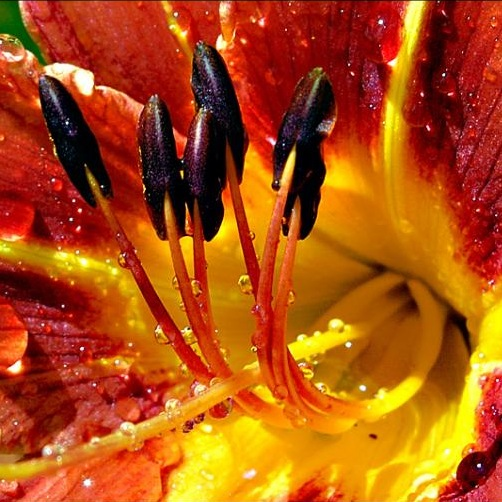
\includegraphics[width=0.3\textwidth]{flowers.png}
	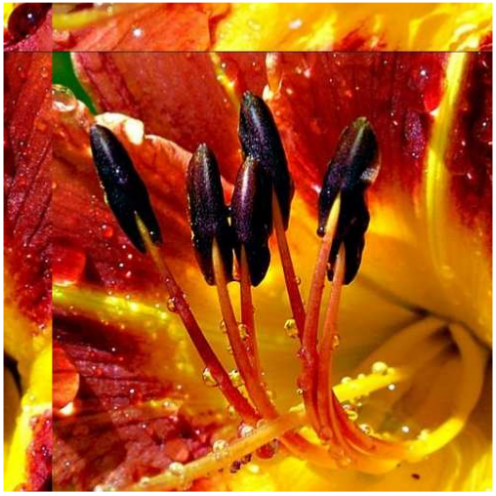
\includegraphics[width=0.3\textwidth]{flowers-translated.png}
	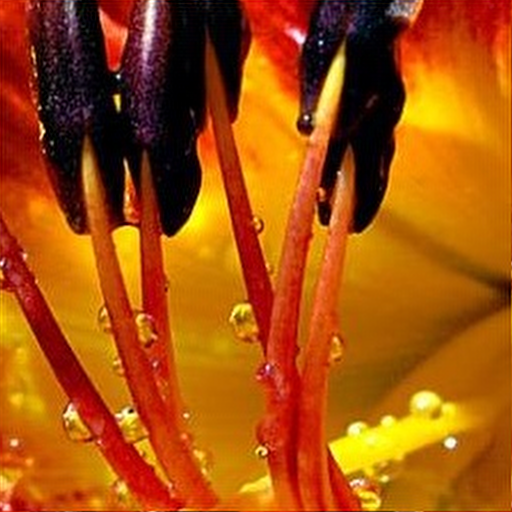
\includegraphics[width=0.3\textwidth]{flowers-zoomed.png}
  \caption{Image originale, translatée et zoomée}
\end{figure}
\begin{thebibliography}{2}

\bibitem{unser95}
  Unser, Michael, Philippe Thevenaz, and Leonid Yaroslavsky. 
  "Convolution-based interpolation for fast, high-quality rotation of images." 
  IEEE Transactions on Image Processing 4.10 (1995): 1371-1381.
\bibitem{larkin97}  
  Larkin, Kieran G., Michael A. Oldfield, and Hanno Klemm. 
  "Fast Fourier method for the accurate rotation of sampled images." 
  Optics communications 139.1 (1997): 99-106.
\bibitem{paeth86}
	Paeth, Alan W. 
	"A fast algorithm for general raster rotation." 
	Graphics Interface. Vol. 86. 1986.

\end{thebibliography}

\end{document}
